\chapter{11.Mathematischer Nachschlag}
Aus mathematischer Sicht sind einige Fragen offen geblieben, etwa:

\newcommand{\D} {
\mathcal{D}
}

\section{Verallgemeinerte Funktionen und Abbleitungen}
Wie differenziert man unstetige Funktionen?

Sei $\D := C_0^\infty(\R^d)$ die Menge (auch ein Vektorraum) der beliebig oft differenzierbaren Funktionen auf $\R^d$ mit beschränktem Träger. Etwa:

\begin{center}
    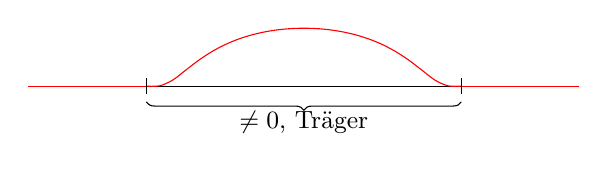
\begin{tikzpicture}
        \draw (-3,0) -- (3,0);
        \draw[scale=2,domain=-0.999:0.999,smooth,variable=\x,red] plot ({\x},{e^(-(1 - abs(\x)^2 )^(-1)});
        \draw[red] (-3.5,0) -- (-0.999*2,0);
        \draw[red] (3.5,0) -- (0.999*2,0);
        \draw (0.999*2,-0.1) -- (0.999*2,0.1);
        \draw (-0.999*2,-0.1) -- (-0.999*2,0.1);
        \draw[decorate,decoration={brace,amplitude=3pt,mirror}] (-2,-0.2) -- node[below] {\small $\neq0$, Träger} (2,-0.2);
    \end{tikzpicture}
\end{center}

Diese Funktion ist:

\[\varphi(x)=g(1- \abs{x}^2)\]

wobei

\[g(t) := \begin{cases}
    e^{\frac{-1}{t}} & ,t>0\\
    0 & ,t\leq 0
\end{cases}\]

Dieses Funktioniert auch im $\R^d$

\def\centerx{2}
\def\centery{-1}

\begin{center}
    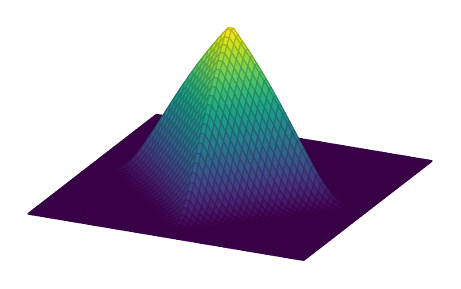
\begin{tikzpicture}[        declare function={
        func(\x) = (\x>0) * e^(-(\x)^(-1)) +
                   (\x<=0) * 0;
      }]

        \pgfplotsset{
            colormap name=viridis,
        }
            \begin{axis}[hide axis,scale=0.75,name=plot1,samples=10]
                \addplot3[surf,domain=-1:1,domain y=-1:1,samples=60]
                    {func(1 - abs(x) - abs(y)))};
                \end{axis}
    \end{tikzpicture}
\end{center}

ist $C_0^\infty(\R^d)$ und hat kompakten Träger.

Sei nun $L^1_{loc}(\R^d)$ die Menge aller Funktionen auf $\R^d$ mit kompaktem Träger für die:

\[\int_K \abs{f(x)} dx < \infty\]

für alle abgeschlossenen und beschränkten Mengen $K \subset \R^d$ gilt.

\begin{center}
    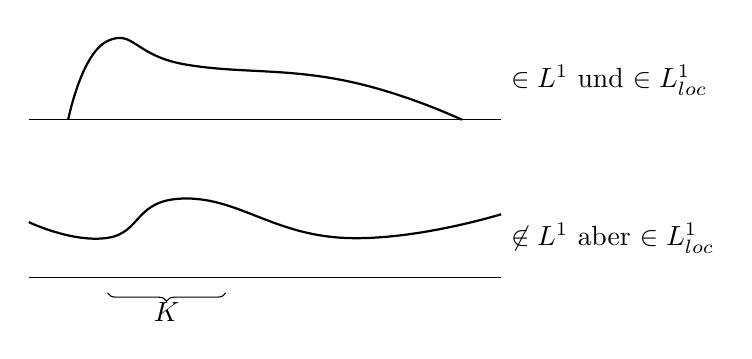
\begin{tikzpicture}
        \draw (-3,0) -- (3,0);
        \draw[thick] plot [smooth, tension = 0.8] coordinates {(-2.5,0) (-2,1)  (-1,0.7) (1,0.5) (2.5,0)};
        \draw (3,0.5) node[right] {$\in L^1$ und $\in L^1_{loc}$};
        \draw (-3,-2) -- (3,-2);
        \draw[thick] plot [smooth, tension = 0.8] coordinates {(-3,-1.3) (-2,-1.5) (-1,-1) (1,-1.5) (3,-1.2) };
        \draw (3,-1.5) node[right] {$\not \in L^1$ aber $\in L^1_{loc}$}; 
        \draw[decorate,decoration={brace,amplitude=3pt,mirror}] (-2,-2.2) -- node[below] {$K$} (-0.5,-2.2);
    \end{tikzpicture}
\end{center}

Die Zweite Funktion ist nicht in $L^1$ da ihr Gesamtintegral nicht endlich ist jedoch ist das Integral über jede endlich Menge endlich, sie hat also keine Pole, somit sie in $L^1_{loc}$.

Für jede Funktion $f \in L^1_{loc}(\R^d)$ bildet 
\begin{equation}\label{eq.11.1}
    \tilde f:\varphi \in \Omega \mapsto \int_{\R^d} f(x) \C \varphi(x) dx \in \R
\end{equation}

ein stetiges lineares Funktional auf $\D$.

Sei nun $\D'$ die Menge aller stetigen linearen Funktionale auf $\D$, also der \mim{Dualraum}. Also ist für jedes $f \in L^1_{loc}$ das Funktional $\tilde f$ aus \eqref{eq.11.1} in $\D'$.

\begin{center}
    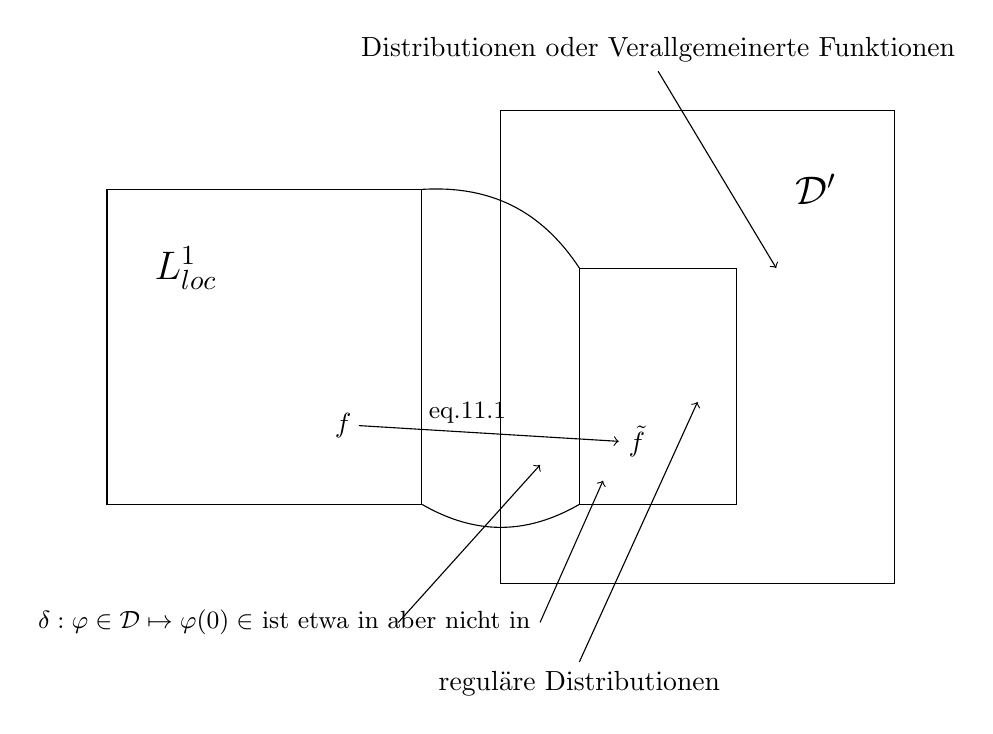
\begin{tikzpicture}
        \draw (0,0) rectangle (4,4);
        \draw (1,3) node[] {\Large $L^1_{loc}$};
        \draw (3,1) node[] {$f$};
        \draw (5,-1) rectangle (10,5);
        \draw (6,0) rectangle (8,3);
        \draw (4,4) to[bend left] (6,3);
        \draw (4,0) to[bend right] (6,0);
        \draw[->] (3.2,1) -- node[above]{\small \eqref{eq.11.1} \ \ \ \ \ } (6.5,0.8) node[right] {$\tilde f$};
        \draw (9,4) node[] {\Large $\D'$};
        \draw[<-] (7.5,1.3) -- (6,-2) node[below]{reguläre Distributionen};
        \draw[<-] (8.5,3) -- (7,5.5) node[above]{\mim{Distributionen} oder Verallgemeinerte Funktionen};
        \draw (-1,-1.5) node[right] {\small $\delta:\varphi \in \D \mapsto \varphi(0) \in \R$ ist etwa in  aber nicht in};
        \draw[<-] (6.3,0.3) -- (5.5,-1.5);
        \draw[<-] (5.5,0.5) -- (3.7,-1.5);
    \end{tikzpicture}
\end{center}

Nun zu den Abbleitungen, sein zunächst $d=1$ und $f \in C^1 \subset L^1_{loc}$, dann gilt für alle $\varphi \in \D$ wobei $[-a,a] \supset supp(\varphi)$:

\[\underbrace{\int_{\R^1} f'(x) \varphi(x) dx}_{f'(\varphi)} = \int_{-a}^a f(x) \phi(x) dx = \underbrace{f(x)\varphi(x)|_{-a}^{a}}_{=0} - \int_{-a}^a f(x) \varphi'(x) dx = -\int_{\R^1} f(x) \varphi'(x) dx = -\tilde f(\varphi')\]

$\Rightarrow$ Für $f \in C^1 \subset L^1_{loc}$ gilt $\tilde f'(\varphi) = - \tilde f(\varphi'), \varphi \in \D$. Wir nehmen dies als Ansatz und setzen:

\begin{equation}\label{eq.11.2}
    F'(\varphi):=-F(\varphi'), \varphi \in \D
\end{equation}

für alle $F\in \D$, genannt Distributionen Abbleitung.

Beispiel:

\begin{center}
    \begin{tikzpicture}
        \draw (-0.4,0) node[left] {$f(x) = \abs{x}$};
        \draw (-0.2,0) -- (4.2,0);
        \draw[thick] (0,2) -- (2,0) -- (4,2);
        \draw (2,-0.1) -- (2,2.3);
    \end{tikzpicture}
\end{center}
Und $F:=\tilde f$ also:

\[F'(\varphi) = -F(\varphi) = - \int_{-a}^a \abs{x} \varphi'(x) dx = - \int_{-a}^0 -x \varphi'(x) dx - \int_0^a x \varphi'(x) dx \]

\[= \int_{-a}^0 x \varphi'(x) dx - \int_0^a x \varphi'(x) dx = \underbrace{x \varphi(x)|_{-a}^0}_{0} - \int_{-a}^0 1 \varphi(x) dx - \underbrace{x \varphi(x)|_0^a}_{0} + \int_0^a 1 \varphi(x) dx\]

\[= \int_{-a}^a sing(x) \varphi(x) dx = \tilde{sign}(\varphi)\]

\begin{center}
    \begin{tikzpicture}
        \draw (-0.4,0) node[left] {$sign(x)=$};
        \draw (-0.2,0) -- (4.2,0);
        \draw (2,-1.3) -- (2,1.3);
        \draw[thick] (2,1) node[left]{\small $1$} -- (4,1);
        \draw[thick] (0,-1) -- (2,-1) node[right]{\small $-1$};
    \end{tikzpicture}
\end{center}

Also insgesamt $F'=\tilde{sign}$

Nun leiten wir die $sign$ Funktion nocheinmal ab:

\begin{align*}
    \tilde{sign}'(\varphi) =& -\tilde{sign}(\varphi') = - \int_\R sign(x) \varphi'(x) dx = - \int_{-a}^a sign(x) \varphi'(x) dx\\
    =&- \int_{-a}^0 (-1) \varphi'(x) dx - \int_0^a 1 \varphi'(x)dx\\
    =&\underbrace{\int_{-a}^0 \varphi'(x) dx}_{\varphi(0) - \varphi(-a)} - \underbrace{\int_0^a \varphi'(x)dx}_{-\varphi(a)+\varphi(0)} = 2 \varphi(0) = 2 \delta(\varphi)\\
    \Rightarrow & \tilde{sign}'=2\delta
\end{align*}

Diese Abbleitung ist jedoch nicht mehr mit einem Element in $L^1_{loc}$ identifizierbar.
Distributionen sind beliebig oft differenzierbar, somit folgt:

\[F^{(k)}(\varphi) = (-1)^kF(\varphi^{(k)}\]

Ein anderes Beispiel in mehr Dimensionen:

Hier ist die Abbleitung definiert über:

\[(D^\alpha F)(\varphi) = (-1)^{\abs{\alpha}}F(D^{\alpha} \varphi), \quad \varphi \in \mathcal{D}, \alpha \in \N^d\]

Für dieses Beispiel ist $d=2$ und $\alpha = \mat{2\\1}$, wobei $\abs{\alpha} = \alpha_1 + ... +\alpha_d$.

\[\Rightarrow D^\alpha = \frac{\partial^{\alpha_1}}{(\partial x_1)^{\alpha_1}}\frac{\partial^{\alpha_2}}{(\partial x_2)^{\alpha_2}} = \frac{\partial^{2}}{(\partial x_1)^{2}} \frac{\partial}{\partial x_2}\]

also

\[(\underbrace{D^\alpha F}_{F_{x_1 x_1 x_2}})(\varphi) = (-1)^{3}F(\varphi_{x_1 x_1 x_2})\]

$\abs{\alpha}=1 \Rightarrow $ eine partielle Abbleitung $\Rightarrow$ Gradient, also Vektor der $1.$ partiellen Abbleitungen.

\subsection{Verallgemeinerter Gradient und Totalvariation}

Für $f:\R^d \to \R$ erwarten wir $\nabla f = \srmatrix{f_{x_1} \\ \vdots \\ f_{x_2}}$

Nun fassen wir jede Komponente $f_{x_1}$ als Distribution auf:

\[\tilde{\nabla f} \coloneqq \mat{\tilde{f_{x_1}}\\ \vdots \\ \tilde{f_{x_d}}}: \mat{\varphi_1 \\ \vdots \\ \varphi_d} \mapsto \underbrace{\tilde{f_{x_1}}(\varphi_1) + \hdots + \tilde{f_{x_1}}(\varphi_1)}_{\in \R}\]

Mit \eqref{eq.11.2} ergibt sich:

\begin{equation}\label{eq.11.3}
    \nabla f(\varphi)=\sum_{k=1}^d \tilde{f_{x_k}}(\varphi_k) \overset{\eqref{eq.11.2}}{=} \sum_{k=1}^d - \tilde{f}\left(\frac{\partial}{\partial x_k} \varphi_k \right) = -\tilde{f} \left( \sum_{k=1}^d \frac{\partial}{\partial x_k} \varphi_k \right) = - \tilde f (div(\varphi)), \ \varphi \in \D^d
\end{equation}

genannt \mim{Distributioneller Gradient}. Das heißt $\tilde{\nabla f}$ ist eine lineare Abbildung von $\D^d \to \R$.

Die Totalvariation von $f \in L^1_{loc}$ ist die Operatornorm dieses Funktionals $\tilde{\nabla f}:(\D^d,\norm{\cdot}_\infty) \to \R$

\begin{equation}\label{eq.11.4}
    TV(f) \coloneqq \underset{\varphi \in \D^d, \norm{\varphi}_\infty = 1}{sup} \bigl| \tilde{\nabla f}(\varphi)\bigr| \overset{\eqref{eq.11.3}}{=} TV(f) \coloneqq \underset{\varphi \in \D^d, \norm{\varphi}_\infty = 1}{sup} \tilde{f}(div(\varphi))
\end{equation}

Für folgende Spezialfälle wird  $TV(\varphi)$ etwas handlicher als in \eqref{eq.11.4}:

\begin{enumerate}
    \item Sei $f \in C^1(\Omega)$, d.h. stetig differenzierbar auf $\Omega \subset \R^d$ und $r \in \R^d$ mit $\norm{r}=1$. Für die Richtungsabbleitung $\frac{\partial f}{\partial r}$ gilt:

    \[\frac{\partial f}{\partial r} = \skprod{\nabla f(x)}{r} \leq \norm{\nabla f(x)} \C \underbrace{\norm{r}}_{1} = \norm{\nabla f(x)}\]

    mit Gleichheit im Falle von $r = \frac{\nabla f(x)}{\norm{\nabla f(x)}}$.
    
    Es ergibt sich:

    \begin{align}\label{eq.11.5}
        TV(f) &= \underset{\varphi \in \D^d, \norm{\varphi}_\infty = 1}{sup} \bigl(\tilde{f_{x_1}}(\varphi_1) + ... + \tilde{f_{x_d}}(\varphi_d)\bigr) \nonumber \\
        &= \underset{\varphi \in \D^d, \norm{\varphi}_\infty = 1}{sup} \underbrace{\int_\Omega f_{x_1}\varphi_1(x) + ... + f_{x_d}(x)\varphi_d(x) dx}_{\skprod{\nabla f(x)}{\varphi(x)}} = \int_\Omega \norm{\nabla f(x)} dx
    \end{align}

    Dabei wird immer $\varphi(x) = \frac{\nabla f(x)}{\norm{\nabla f(x)}}$ gewählt, was zwar im Allgemeinen nicht in $\D^d$ liegt, sich aber beliebig gut approximieren lässt.

    \item Sei $f= \chi_D$ die charakteristische Funktion con $D \subset \Omega \subset \R^d$, wobei $D$ beschränkt sei und stückweise glatten Rand besitzt.
    Dann gilt:

    \[\tilde{\nabla f}(\varphi) \overset{\eqref{eq.11.3}}{=} - \int \chi_D div(\varphi(x)) dx \overset{\text{\small{Gaußscher Integralsatz}}}{=} -\int_{\partial D} \skprod{\varphi(x)}{n(x)} ds(x)\]
    
    wobei $n(x)$ der Normalenvektor an $\partial D$ ist.

    \begin{align}
        \Rightarrow TV(f) =& \underset{\varphi \in \D^d, \norm{\varphi}_\infty = 1}{sup} \int_{\partial D} \skprod{\varphi(x)}{n(x)} ds(x) \nonumber \\
        =& \int_{\partial D}\underbrace{\norm{n(x)}}_{1} ds(x) = \int_{\partial D} 1 ds(x) = \text{Länge}(\partial D)
    \end{align}
\end{enumerate}

\subsection{Existenz und Eindeutigkeit der Variationslösung}
Wann ist ein Minimierungsproblem:

\[J(u) \overset{u \in U}{\longrightarrow}\]

eindeutig lösbar?

\begin{enumerate}
    \item Existenz 
    \[J:U\to \R\]
    Wobei $U$ ein metrischer Raum ist.

    Aus der Analysis ist bekannt, dass stetige Funktionen auf kompakten Mengen ihr Maximum und Minimum annehmen.

    \begin{minipage}[c]{0.49\textwidth}
        
        \begin{center}
            \begin{tikzpicture}
                \draw (-1,0) -- (4,0);
                \draw (0,3) -- (0,-1);
                \draw[{)-*},thick] (0,0) -- (4,0);
                \draw (2,0) node[below] {\small nicht kompakt};
                \draw (-0.2,0) node[below] {\small $0$};
                \draw (4,0) node[below] {\small $1$};
                \draw[scale=0.75,domain=0.25:5.3,thick,smooth,variable=\x,samples=500] plot ({\x},{1/\x});
                \draw[)-,thick] (0,2) -- (4,0.5);
            \end{tikzpicture}
        \end{center}

        \end{minipage}
        \begin{minipage}[c]{0.49\textwidth}
        Nimmt sei Maximum \underline{nicht} an, da $U$ nicht kompakt ist, jedoch ist $f$ stetig.
    \end{minipage}


    \begin{minipage}[c]{0.49\textwidth}
        
        \begin{center}
            \begin{tikzpicture}
                \draw (-1,0) -- (4,0);
                \draw[,thick] (0,0) -- (3,0);
                \draw (1.5,0) node[below] {\small kompakt};
                \draw (0,0.1) -- node[below] {0} (0,-0.1);
                \draw (3,0.1) -- node[below] {1} (3,-0.1);
                \draw[*-(] (0,0.3) -- (2,1.5);
                \draw[*-*] (2,0.3) -- (3,1);
            \end{tikzpicture}
        \end{center}

        \end{minipage}
        \begin{minipage}[c]{0.49\textwidth}
        Nimmt sei Maximum \underline{nicht} an, da $f$ unstetig ist, jedoch ist $U$ kompakt.
    \end{minipage}

    Wir benötigen jedoch nur die Existenz des Minimums, nicht des Maximums, daher reicht im obigen Satz die \mim{Untere Halbstatigkeit}, diese ist für ein $u_0 \in U$ erfüllt falls:

    \[\forall \epsilon > 0 \ \exists \delta: J(U_\delta(u_0)) \subset \left( J(u_0), \infty \right)\]

    Im Vergleich zur gewöhnlichen Stetigkeit:

    \[\forall \epsilon > 0 \ \exists \delta : J(U_\delta (u_0)) \subset U_\epsilon (J(u_0))\]

    Aber auch die Kompaktheit vun $U$ ist nicht oft erfüllt, deshalb definieren wir:
    
    \[S_\alpha  \coloneqq \{ u \in U : J(u) \leq \alpha \}, \quad \text{\mim{Sub-Niveaumenge} zu Niveu $\alpha$} \]

    \textbf{Existenzsatz}: Sei $U$ ein metrischer Raum und 

    \[J:U \to \R\]
    so dass:

    \begin{enumerate}
        \item $J$ unter-halbstetig
        \item $\exists \alpha \in \R : S_\alpha \neq \emptyset$ und kompakt
    \end{enumerate}

    Dann existiert ein Minimierer $u^* \in U$ mit:

    \[J(u^*) \leq J(u) \quad \forall u \in U \]

    \item Eindeutigkeit

    \begin{minipage}[c]{0.34\textwidth}
        
        \begin{center}
            \begin{tikzpicture}
                \draw (0,0) -- (5,0);
                \draw[name path=A] plot [smooth,tension=1] coordinates {(0.25,0.75) (2.5,0.2)  (4.75,1.5)};
                \draw (0.5,0.1) -- node[below] {\small $u$} (0.5,-0.1);
                \draw (4.5,0.1) -- node[below] {\small $v$} (4.5,-0.1);
                \draw[draw =none,name path=B] (0.5,1) -- (0.5,0);
                \draw[draw =none,name path=C] (4.5,1.5) -- (4.5,0);
                \path[name intersections={of=A and B,by=D}];
                \path[name intersections={of=A and C,by=E}];
                \draw[name path = F] (D) -- (E);
                \fill (D) circle[radius = 1.5pt];
                \fill (E) circle[radius = 1.5pt];
                \draw[draw = none, name path = G] (3,1.5) -- (3,0);
                \path[name intersections={of=F and G,by=H}];
                \path[name intersections={of=A and G,by=I}];
                \fill[red] (H) circle[radius = 1.5pt];
                \fill (I) circle[radius = 1.5pt];
                \draw[dotted] (H) -- (3,0);
                \draw (3,0.1) -- (3,-0.1) node[below] {\small $\alpha u + (1- \alpha)v$};
            \end{tikzpicture}
        \end{center}

        \end{minipage}
        \begin{minipage}[c]{0.65\textwidth}
        $J:U \to \R$ heißt \mim{strengkonvex} falls $\forall u,v \in U, \ \alpha \in (0,1)$:

        \[\underbrace{J(\alpha u + (1-\alpha)v)}_{\text{\textbullet}} < \underbrace{\alpha J(u) + (1-\alpha) J(v)}_{\color{red} \text{\textbullet}} \]
    \end{minipage}

    \textbf{Eindeutigkeitssatz}: Falls $J$ strengkonvex ist existiert höchstens ein Minimierer.

    \begin{proof}
        Angenommen, $u^* \neq v^*$ seien Minimierer von $J$, d.h.

        \[\alpha_{\text{min}} \coloneqq J(u^*) = J(v^*) \leq J(u) \quad \forall u \in U\]

        \[\overset{\text{\small str. konvex}}{\Longrightarrow} \forall \alpha \in (0,1) : J(\alpha u^* + (1 - \alpha)v^*) < \alpha J(u^*) + (1-\alpha)J(v^*) = \alpha_{\text{min}} \ \lightning \]

        Dieses ist jedoch ein Widerspruch zur Minimalität von $J(u^*)$ und $J(v^*)$.

    \end{proof}

\end{enumerate}